\documentclass[12pt]{article}
\usepackage{amsmath}
%\usepackage[lmargin = 0.5in, rmargin = 0.5in, tmargin = 0.5in, bmargin = 0.5in]{geometry}
\usepackage[none]{hyphenat}
\usepackage{graphicx}
\usepackage{float}

\title{\textbf{MAE598/494 Design Optimization\\Homework 1}}
\author{Aditya Vipradas \\ ASU ID: 1209435588}
\begin{document}
\pagenumbering{gobble}
\maketitle
\textbf{Problem 1.a)}\\\\
Use initial point: x0 = (2, 2, 2, 2, 2) to solve:\\\\
minimize: \\$(x1 - x2)^{2} + (x2 + x3 - 2)^{2} + (x4 - 1)^{2} + (x5 - 1)^{2}$\\\\
subject to: \\$x1 + 3x2 = 0$\\$x3 + x4 - 2x5 = 0$\\$x2 - x5 = 0$\\$-10 <= xi <= 10, i = 1,...,5$\\\\\\
(Refer next page for solution using the Excel Solver and Matlab's \emph{fmincon} solver.)
\newpage
\textbf{Problem 1.b)}\\\\
Use initial point: x0 = (1, 1, 1, 1) to solve:\\\\
minimize: \\$24.55x1 + 26.75x2 + 39.00x3 + 40.50x4$\\\\
subject to: \\$2.3x1 + 5.6x2 + 11.1x3 + 1.3x4 - 5 >= 0$\\$12x1 + 11.9x2 + 41.8x3 + 52.1x4 - 21 - 1.645(0.28x1^{2} + 0.19x2^{2} + 20.5x3^{2} + 0.62x4^{2})^{1/2} >= 0$\\$x1 + x2 + x3 + x4 - 1 = 0$\\$0 <= xi, i = 1,...,4$\\\\\\
(Refer next page for solution using the Excel Solver and Matlab's \emph{fmincon} solver.)
\newpage
\textbf{Problem 2}\\\\
Optimization problem to design a cylindrical cola can of volume $V$:
\begin{enumerate}
\item \emph{Design variables:} radius of top face of the can $(r)$ and height of the can $(h)$
\item \emph{Objective function:} minimize the material usage in the cola can by minimizing its surface area i.e. $S = 2 \pi r h + 2 \pi r^{2}$
\item \emph{Constraints:} volume of the can = $V$ i.e. $\pi r^{2} h = V$, $r, h > 0$
\item \emph{Assumptions:} 
\begin{enumerate}
\item The cola can is assumed to have negligible thickness
\item The cola can is assumed to be perfectly cylindrical i.e. without any opening, surface defects and dents
\end{enumerate}
\end{enumerate}
Assume the volume of a standard Coca Cola can to be $V = 355 mL$. Solving the optimization problem by substituting $V/(\pi r^{2})$ for h from the constraint equation in the objective function. Consequently, differentiating the objective function in $r$ with respect to $r$ and equating to zero, the relation $2r = h$ is obtained. Thus, in order to minimize the material usage in a cola can, for a given volume $V$, the radius $r$ of the top face should be half of that of its height $h$. The dimensions of a standard $355 mL$ Coca Cola are approximately as follows:
\begin{figure}[ht]
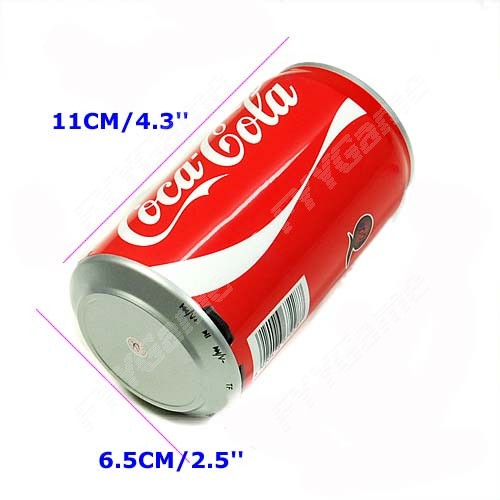
\includegraphics[scale=0.3]{img.jpg}
\end{figure}

As observed, for a given diameter of $6.5 cm$, the height of the can is $11 cm$. But from the relation obtained above i.e. $2r = h$, for a volume of $355 mL$, the height and diameter of the can should be 7.67 cm. Thus, the obtained optimal solution is not close to the reality. The practical reasons for this are as follows:
\begin{enumerate}
\item The dimensions of the cola can should be ergonomic. The consumer should be able to grasp the can in his hand. It would be cumbersome for the user to hold a can 7.67 cm long using all his fingers. Hence, the height is generally bigger than the can diameter, here 11 cm for the user to easily hold it in his hand. 
\item If not negligible, the cola can has some finite thickness which will increase the surface area and in turn the material usage. 
\item Moreover, the base of the can is not perfectly flat. It has a dent for it to get perfectly located on the can tray. The top face is also not flat. It has extra material that goes in the opener. Thus, more material than the one predicted by the optimal solution is used to manufacture the cola can.
\item Furthermore, the can has to sustain the pressure produced in it. Thus, additional material than the one obtained from the optimal solution is used in the appropriate locations to preserve its strength.
\end{enumerate}
\end{document}
